\documentclass[11pt, reqno]{amsart}

\input{~/latex-common/macros.tex}
\usepackage[backend=bibtex,style=science]{biblatex}
% \bibliography{main.bib}
\pgfplotsset{compat=1.18}

\pagestyle{fancy}                         % fancy (allow headers, footers)
\fancyhf{}                                % clear all header/footer settings.
\cfoot{\thepage}                          % set page-numbers in footer.
% \lhead{\textit{\textbf{ Amittai, S}}}   % set name in header, left.
% \rhead{\textsc{Math 71: Algebra}}       % set class name in header, right.
\renewcommand{\headrulewidth}{0pt}
\renewcommand{\footrulewidth}{0pt}


\renewcommand{\theenumi}{\alph{enumi}}

\begin{document}

\newdate{due-date}{05}{04}{2023}

\title{CS-49: Game Theory\\ Amittai Siavava \\ \displaydate{due-date}}
\author{Amittai Siavava}
% \date{\today}


\setlength{\headheight}{13.0pt}
\setlength{\footskip}{15.0pt}

\maketitle

\begin{problem}[4]
  \emph{Read \textbf{Chapter $0$} of Lessons in Play, and do \textbf{Problem $1$} at the end of the chapter.}

  \step
  Consider the position:

  \begin{enumalph}
    \item Draw the complete game trees for both \textsc{cram}
      and \textsc{domineering}. The leaves (bottoms) of the tree
      should all be positions in which neither player can move.
      If two left (or right) options are symmetrically identical, you may omit one.

      \begin{figure}[H]
        
        % Draw an empty 3x4 chessboard.
        % Remove the arrow
        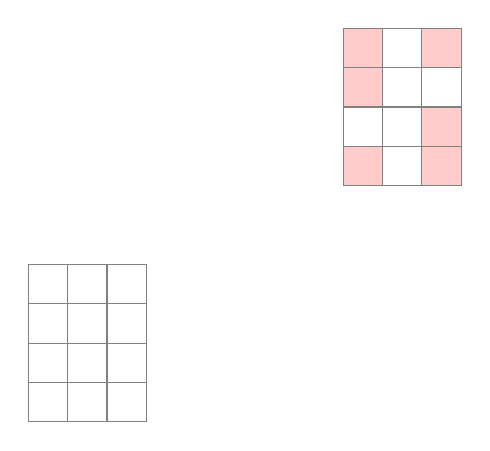
\begin{tikzpicture}[scale=0.5]
          % draw a 3 x 4 grid at (0,0), fill the first square
          \fill[red!20](0,0) rectangle (1,-2);
          \fill[red!20](0,-3) rectangle (1,-4); 

          \fill[red!20](2,0) rectangle (3,-1);
          \fill[red!20](2,-2) rectangle (3,-4);

          \draw[step=1cm,gray] (0,0) grid (3,-4);


          % \draw[step=1cm,gray] (0,0) grid (3,-4);

          \draw[step=1cm,gray] (-8,-6) grid (-5,-10);

          % draw edge 


        \end{tikzpicture}
      \end{figure}

    \item Who wins at \textsc{domineering} if Vertical plays first?
      Who wins if Horizontal plays first? Who wins at \textsc{cram}?
  \end{enumalph}
\end{problem}
\end{document}
